\section{\textcolor{Salmon}{Überblick und Aufbau der bestehenden Ergebnisanzeige}}
\label{ch:IST-Zustand:sec:Aufbau_altes_System}

Das System zur Ergebnisanziege des Testpools besteht aus verschiedenen Oberflächen, die jeweils einen Anwendungsfall darstellen. \autoref{fig:aufbau_altes_System} ist ein Ausschnitt aus der Oberfläche, in dem die Testergebnisse dargestellt sind. Außerhalb von sind Dropdown-Menüs zu finden, in den die Attribute wie beispielsweise der Maschinenname und Versionsnummer. Die Oberflächen sind weiterhin über einen internen Link zugänglich, in dem ebenfalls alle Attribute zur Identifikation angegeben sind.

\begin{figure}[H]
    \centering
    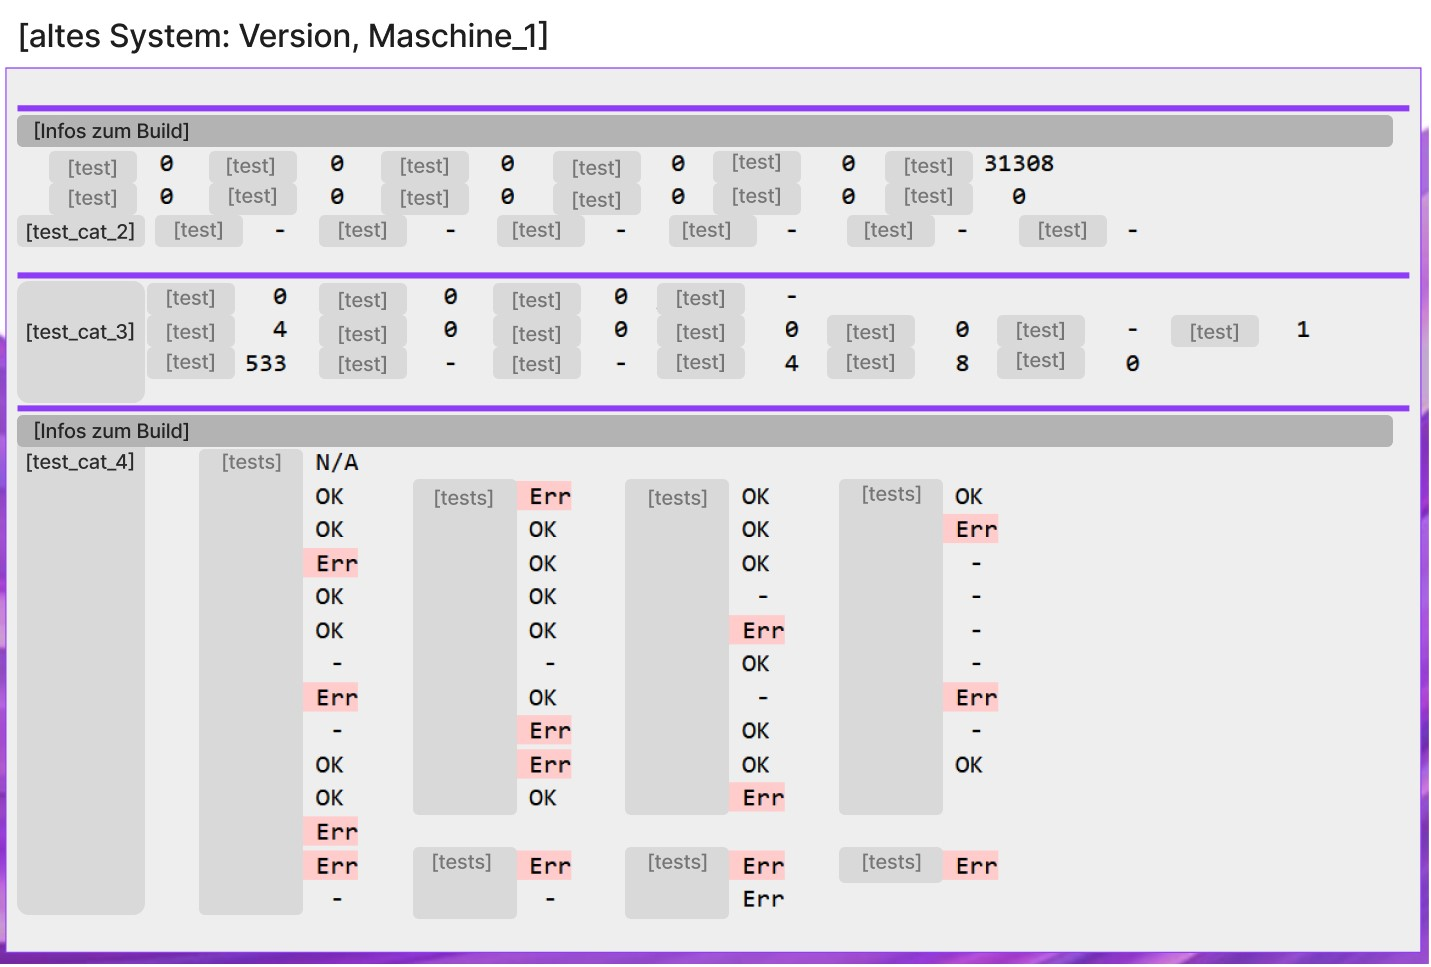
\includegraphics[width=1\linewidth]{Dashboard/altesSystem_zensiert.jpg}
    \caption{Aufbau des alten Systems [zensiert]}
    \label{fig:aufbau_altes_System}
\end{figure}

\noindent
\underline{Auf dem Bild erkennbar (s. \autoref{fig:aufbau_altes_System})}\\
Name des Kontexts\\
Build-Infos\\
Test-Kategorien in Zeilen\\
Testumgebungen / -namen jeweils in Spalten - den Zeilen zugeordnet\\
-> zusammengefasstes Testergebnis daneben\\
--> Test-Kategorie 1,2,3: Anzahl der Fehler als Zahlwert oder Kürzel für 'Absturz im Bauprozess'\\
--> Test-Kategorie 4: Auflistung des Zustands (Ok, Err (Fehler), - (noch nicht gelaufen) oder Crash)

\noindent
\underline{\autoref{fig:aufbau_altes_System}:}\\
\textcolor{red}{Begründung Zensur}\\
-> \textcolor{red}{TODO: Marcus}
